\documentclass[aspectratio=169]{beamer}
\usepackage{fontspec}
\usepackage{graphicx}
\usepackage{tikz}
\usepackage{xcolor}
\usetikzlibrary{calc}  

% Define custom color
\definecolor{vyperblack}{HTML}{180C25}
\definecolor{vyperviolet}{HTML}{9F4CF2}
\definecolor{bubblecolor}{HTML}{DDCEAF}
\definecolor{numbertextcolor}{HTML}{FDFCFB}


% Set Inconsolata as the main font and for all text elements
\setmainfont{Inconsolata}[
Path = /usr/share/fonts/TTF/,
Extension = .ttf,
UprightFont = *-Regular,
BoldFont = *-Bold,
ItalicFont = *-Regular,
BoldItalicFont = *-Bold
]
\setsansfont{Inconsolata}[
Path = /usr/share/fonts/TTF/,
Extension = .ttf,
UprightFont = *-Regular,
BoldFont = *-Bold,
ItalicFont = *-Regular,
BoldItalicFont = *-Bold
]

% Set SemiExpanded Bold for titles
\newfontfamily\titlefont{Inconsolata}[
Path = /usr/share/fonts/TTF/,
Extension = .ttf,
UprightFont = *_SemiExpanded-Bold,
BoldFont = *_SemiExpanded-Bold,
ItalicFont = *_SemiExpanded-Bold,
BoldItalicFont = *_SemiExpanded-Bold
]

% Set theme
\usetheme{default}
\usecolortheme{default}

% Remove navigation symbols
\setbeamertemplate{navigation symbols}{}

% Custom background
\setbeamertemplate{background}{
	
\includegraphics[width=\paperwidth,height=\paperheight]{supergraphic.png}
}

% Custom title page
\setbeamertemplate{title page}{
	\begin{tikzpicture}[remember picture,overlay]
		\node[anchor=north west,yshift=-20pt,xshift=20pt] at (current page.north west) {
			
\includegraphics[width=0.25\textwidth]{vyper-logo-landscape-color-pos.pdf}
		};
		\node[anchor=north west,yshift=-20pt,xshift=20pt] at (current page.north west) {
			\parbox{0.95\textwidth}{\vspace{3.25cm}\raggedright\fontsize{40}{48}\selectfont\titlefont\textcolor{vyperblack}{\textbf{\inserttitle}}}
		};
	\end{tikzpicture}
}

% Custom frame title
\setbeamertemplate{frametitle}{
	\begin{tikzpicture}[remember picture,overlay]
		\node[anchor=north west,yshift=-10pt,xshift=10pt] at (current page.north west) {
			
\includegraphics[width=0.04\textwidth]{VYPER_SYMBOL_COLOR.png}
		};
		\node[anchor=north west,yshift=-10pt,xshift=0.11\textwidth] at (current page.north west) {
			\parbox{0.94\textwidth}{\raggedright\fontsize{24}{26}\titlefont\textcolor{vyperblack}{\textbf{\insertframetitle}}}
		};
	\end{tikzpicture}
}

% Set all text to vyperblack
\setbeamercolor{normal text}{fg=vyperblack}
\setbeamercolor{frametitle}{fg=vyperblack}
\setbeamercolor{title}{fg=vyperblack}

\title{Vyper Roadmap \\ Growth \& Funding}

\begin{document}
	
	% Title slide
	\begin{frame}[plain]
		\titlepage
	\end{frame}
	
	% Second slide - KPI
	\begin{frame}
		\frametitle{Vyper at a Glance}
		\begin{columns}[T,totalwidth=\textwidth]
			\begin{column}{0.5\textwidth}
				\begin{center}
					\textcolor{vyperviolet}{\fontsize{40}{48}\selectfont\textbf{\$4.1b}}
					\vspace{0.5em}
					
					\small Total Value Locked\\in Vyper Contracts
				\end{center}
			\end{column}
			\begin{column}{0.5\textwidth}
				\begin{center}
					\textcolor{vyperviolet}{\fontsize{40}{48}\selectfont\textbf{2\textsuperscript{nd}}}
					\vspace{0.5em}
					
					\small Most popular EVM language
				\end{center}
			\end{column}
		\end{columns}
		
		\vspace{1em}
		
		\begin{columns}[T,totalwidth=\textwidth]
			\begin{column}{0.5\textwidth}
				\begin{center}
					\textcolor{vyperviolet}{\fontsize{40}{48}\selectfont\textbf{10}}
					\vspace{0.5em}
					
					\small New Vyper contracts\\deployed every day
				\end{center}
			\end{column}
			\begin{column}{0.5\textwidth}
				\begin{center}
					\textcolor{vyperviolet}{\fontsize{40}{48}\selectfont\textbf{100+}}
					\vspace{0.5em}
					
					\small Contributors on Github
				\end{center}
			\end{column}
		\end{columns}
	\end{frame}
	
	% Third Slide - Protocols using Vyper
	\begin{frame}
		\frametitle{They use Vyper}
		\centering
		\begin{tikzpicture}[remember picture,overlay]
			% Top row
			\foreach \x/\name in {0/Curve, 1/Frax, 2/Lido, 3/{Perpetual Protocol}}
			{
				\node[anchor=north] at ($(current page.north)+(-0.375\paperwidth+0.25\paperwidth*\x,-0.18\paperheight)$) {
					\includegraphics[width=0.12\paperwidth]{users/\name.png}
				};
				\node[anchor=north, text width=0.18\paperwidth, align=center] at ($(current page.north)+(-0.375\paperwidth+0.25\paperwidth*\x,-0.43\paperheight)$) {
					\large\name
				};
			}
			
			% Bottom row
			\foreach \x/\name in {0/Velodrome, 1/Yearn, 2/{Sorella Labs}}
			{
				\node[anchor=north] at ($(current page.north)+(-0.25\paperwidth+0.25\paperwidth*\x,-0.56\paperheight)$) {
					\includegraphics[width=0.12\paperwidth]{users/\name.png}
				};
				\node[anchor=north, text width=0.18\paperwidth, align=center] at ($(current page.north)+(-0.25\paperwidth+0.25\paperwidth*\x,-0.86\paperheight)$) {
					\large\name
				};
			}
		\end{tikzpicture}
	\end{frame}
	
	% Fourth Slide - Vision
	\begin{frame}
		\frametitle{Vision}
		\setbeamercolor{itemize item}{fg=vyperviolet}
		\setbeamercolor{itemize subitem}{fg=vyperviolet}
		\setbeamercolor{itemize subsubitem}{fg=vyperviolet}
		\begin{itemize}
			\item Despite a growing user base and adoption by major DeFi protocols, \textbf{Vyper contracts account for less than 1\% of all new contract deployments}.
			\vspace{1em}
			\item We want to bring this number to \textbf{50\% by 2028.}
			\vspace{1em}
			\item This is the only path to achieve language diversity on Ethereum.
		\end{itemize}
	\end{frame}
		
	% Fifth Slide - User Acquisition
	\begin{frame}
		\frametitle{User Acquisition Pathways}
		\begin{tikzpicture}[remember picture,overlay]
			% First bubble - Converting Developers
			\node[anchor=north west, 
			fill=bubblecolor!70, 
			opacity=0.5,
			rounded corners, 
			text width=0.375\paperwidth,
			inner sep=15pt,
			minimum height=13em] 
			at ($(current page.north west)+(0.04\paperwidth,-0.25\paperheight)$) 
			(bubble1) {};
			
			\node[circle, 
			fill=vyperviolet, 
			text=numbertextcolor, 
			font=\bfseries, 
			minimum size=1.5em] 
			at ($(bubble1.north west)+(0.5em,-0.5em)$) 
			{1};
			
			\node[anchor=north west, 
			font=\bfseries, 
			text width=0.4\paperwidth] 
			at ($(bubble1.north west)+(2em,-0.5em)$) 
			{Converting Developers};
			
			\node[anchor=north west, 
			text width=0.4\paperwidth] 
			at ($(bubble1.north west)+(0.5em,-2.5em)$) 
			{
				\setbeamercolor{itemize item}{fg=vyperviolet}
				\begin{itemize}
					\item Experienced Solidity developers switching to Vyper for their next project
					\vspace{0.5em}
					\item Protocols written in Solidity adding new contracts written in Vyper
				\end{itemize}
			};
			
			% Second bubble - Onboarding Developers
			\node[anchor=north west, 
			fill=bubblecolor!70, 
			opacity=0.5,
			rounded corners, 
			text width=0.375\paperwidth,
			inner sep=15pt,
			minimum height=13em] 
			at ($(current page.north west)+(0.53\paperwidth,-0.25\paperheight)$) 
			(bubble2) {};
			
			\node[circle, 
			fill=vyperviolet, 
			text=numbertextcolor, 
			font=\bfseries, 
			minimum size=1.5em] 
			at ($(bubble2.north west)+(0.5em,-0.5em)$) 
			{2};
			
			\node[anchor=north west, 
			font=\bfseries, 
			text width=0.4\paperwidth] 
			at ($(bubble2.north west)+(2em,-0.5em)$) 
			{Onboarding Developers};
			
			\node[anchor=north west, 
			text width=0.4\paperwidth] 
			at ($(bubble2.north west)+(0.5em,-2.5em)$) 
			{
				\setbeamercolor{itemize item}{fg=vyperviolet}
				\begin{itemize}
					\item Bringing experienced Web2 developers to Web3
					\vspace{0.5em}
					\item Becoming the language of choice for all beginner Web3 developers
				\end{itemize}
			};
		\end{tikzpicture}
	\end{frame}
	
	% Converting Developers Slide
	\begin{frame}
	\frametitle{Converting Developers}
	\begin{columns}[T,totalwidth=\textwidth]
		\begin{column}{0.35\textwidth}
			\vspace{2em} % More space below title
			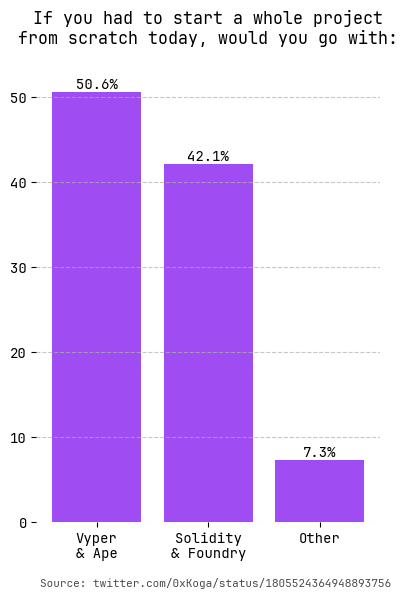
\includegraphics[width=\columnwidth,height=0.75\paperheight,keepaspectratio]{charts/preference.png}
		\end{column}
		\begin{column}{0.65\textwidth}
			\vspace{2em} % More space below title
			\setbeamercolor{itemize item}{fg=vyperviolet}
			\setbeamercolor{itemize subitem}{fg=vyperviolet}
			\setbeamercolor{itemize subsubitem}{fg=vyperviolet}
			\begin{itemize}
				\item 12\% of Solidity developers already also use Vyper (Solidity dev survey 2023) 
				\vspace{0.7em}
				\item Majority of polled developers would pick Vyper over Solidity for their next project
				\vspace{0.7em}
				\item Protocols won't rewrite their codebase in Vyper, but are open to having mixed codebases (Lido, Frax, Velodrome) adding Vyper contracts for new features 
			\end{itemize}
		\end{column}
	\end{columns}
	\end{frame}

% Onboarding Developers Slide
	\begin{frame}
		\frametitle{Onboarding Developers}
		\begin{columns}[T,totalwidth=\textwidth]
			\begin{column}{0.35\textwidth}
				\vspace{2em} % More space below title
				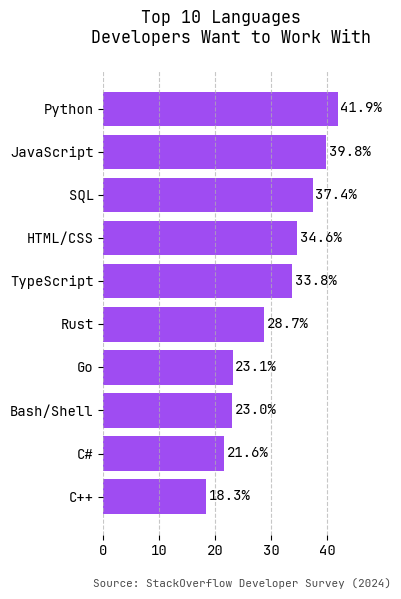
\includegraphics[width=\columnwidth,height=0.75\paperheight,keepaspectratio]{charts/top10.png}
			\end{column}
			\begin{column}{0.65\textwidth}
				\vspace{2em} % More space below title
				\setbeamercolor{itemize item}{fg=vyperviolet}
				\setbeamercolor{itemize subitem}{fg=vyperviolet}
				\setbeamercolor{itemize subsubitem}{fg=vyperviolet}
				\begin{itemize}
					\item Leverage popularity and familiarity of Python among developers
					\vspace{0.7em}
					\item Make Vyper's safety-first design a selling point for beginners
					\vspace{0.7em}
					\item Offer the best developer experience in Web3 with superior tooling, support and integrations
				\end{itemize}
			\end{column}
		\end{columns}
	\end{frame}

	% KPIs Slide
	\begin{frame}
		\frametitle{KPIs}
		\begin{tikzpicture}[remember picture,overlay]
			\foreach \x/\y/\title/\items [count=\i] in {
				0/0/{Deployments}/{- Proportion of new contracts deployed\newline - Total number of contracts deployed},
				1/0/{TVL}/{- Total USD amount secured in Vyper contracts as \% of total crypto TVL},
				0/1/{Github}/{- Github stars for the vyperlang repos\newline - Number of new contributors\newline - Number of repos with Vyper code},
				1/1/{Online Presence}/{- Social media mentions\newline - Engagement metrics for Vyper X account\newline - Unique visitors to website }
			} {
				\node[anchor=north west, 
				fill=bubblecolor!70, 
				opacity=0.5,
				rounded corners, 
				text width=0.4\paperwidth,
				inner sep=10pt,
				minimum height=7em] 
				at ($(current page.north west)+(0.03\paperwidth+0.49\paperwidth*\x,-0.22\paperheight-0.35\paperheight*\y)$) 
				(bubble\i) {};
				
				\node[circle, 
				fill=vyperviolet, 
				text=numbertextcolor, 
				font=\bfseries, 
				minimum size=1.5em] 
				at ($(bubble\i.north west)+(0.5em,-0.5em)$) 
				{\i};
				
				\node[anchor=north west, 
				font=\bfseries, 
				text width=0.4\paperwidth] 
				at ($(bubble\i.north west)+(2em,-0.5em)$) 
				{\title};
				
				\node[anchor=north west, 
				font=\footnotesize, 
				text width=0.4\paperwidth] 
				at ($(bubble\i.north west)+(0.5em,-2.5em)$) 
				{\items};
			}
		\end{tikzpicture}
	\end{frame}
	
	% Bottleneck Slide
	\begin{frame}
		\frametitle{Adoption Bottlenecks}
		\setbeamercolor{itemize item}{fg=vyperviolet}
		\setbeamercolor{itemize subitem}{fg=vyperviolet}
		\setbeamercolor{itemize subsubitem}{fg=vyperviolet}
		
		\vspace{0.51em}
		We have started surveying developers to understand what prevents them from using Vyper. The reasons expressed are \textbf{rarely technical} but instead fall into 2 major categories:
		
		\vspace{1em}
		\begin{itemize}
			\item \textbf{Lack of Awareness}
		\end{itemize}
		\vspace{0.5em}
		\hspace{2em}\parbox{0.8\textwidth}{\footnotesize User has never heard of Vyper. User has heard about it but never tried or looked into it. User is unaware of many of the most recent features. User could not find good tutorials}
		
		\vspace{1em}
		\begin{itemize}
			\item \textbf{Inertia/Reluctance}
		\end{itemize}
		\vspace{0.5em}
		\hspace{2em}\parbox{0.8\textwidth}{\footnotesize User is unwilling to change current workflow/setup. User trusts Solidity because it is the standard. Colleagues/boss do not want to use Vyper}
		
		\vspace{1.5em}
		We believe these can be solved with \textbf{better outreach and communication}.
	\end{frame}
	
	% Action Plan
	\begin{frame}
		\frametitle{Action Plan}
		\begin{tikzpicture}[remember picture,overlay]
			\foreach \x/\y/\title/\items [count=\i] in {
				0/0/{Outreach Hires}/{- Hire a Developer Relations person\newline - Hire a Business Developer\newline - Hire community facing roles},
				1/0/{Communications}/{- Increased social media presence \newline - Increase visibility in web3 media\newline - Improve, regularly update and promote official Vyper website},
				0/1/{Developer Engagement}/{- Ensure presence at major Ethereum events\newline - Partnerships with L2s for Hackathons\newline - Vyper-focused contests},
				1/1/{Developer Experience}/{- Allocate budget to ecosystem tooling\newline - Help tooling projects secure funding\newline - Improve documentation and tutorials}
			} {
				\node[anchor=north west, 
				fill=bubblecolor!70, 
				opacity=0.5,
				rounded corners, 
				text width=0.4\paperwidth,
				inner sep=10pt,
				minimum height=7em] 
				at ($(current page.north west)+(0.03\paperwidth+0.49\paperwidth*\x,-0.22\paperheight-0.35\paperheight*\y)$) 
				(bubble\i) {};
				
				\node[circle, 
				fill=vyperviolet, 
				text=numbertextcolor, 
				font=\bfseries, 
				minimum size=1.5em] 
				at ($(bubble\i.north west)+(0.5em,-0.5em)$) 
				{\i};
				
				\node[anchor=north west, 
				font=\bfseries, 
				text width=0.4\paperwidth] 
				at ($(bubble\i.north west)+(2em,-0.5em)$) 
				{\title};
				
				\node[anchor=north west, 
				font=\footnotesize, 
				text width=0.4\paperwidth] 
				at ($(bubble\i.north west)+(0.5em,-2.5em)$) 
				{\items};
			}
		\end{tikzpicture}
	\end{frame}
	
	% Funding overview
	\begin{frame}
		\frametitle{Funding}
		\setbeamercolor{itemize item}{fg=vyperviolet}
		\setbeamercolor{itemize subitem}{fg=vyperviolet}
		\setbeamercolor{itemize subsubitem}{fg=vyperviolet}
		
		\begin{itemize}
			\item Acquiring users is \textbf{costly} and requires funding
		\end{itemize}
		
		\vspace{1em}
		\begin{itemize}
			\item We see two main sources of funding for Vyper: \textbf{grant funding} (secured with no obligation for the team to provide anything in exchange) and \textbf{commercial funding} (requiring the team to produce a service or product in exchange)
			
		\end{itemize}
		
		\vspace{1em}
		\begin{itemize}
			\item While we are planning for the eventuality of having to offer commercial services, we currently \textbf{favor and prioritize grants} as they make it easier to preserve the neutrality of the language
		\end{itemize}
		
	\end{frame}

	% Revenue Slide
	\begin{frame}
		\frametitle{Funding Sources (Grants)}
		\begin{columns}[T,totalwidth=\textwidth]
			\begin{column}{0.4\textwidth}
				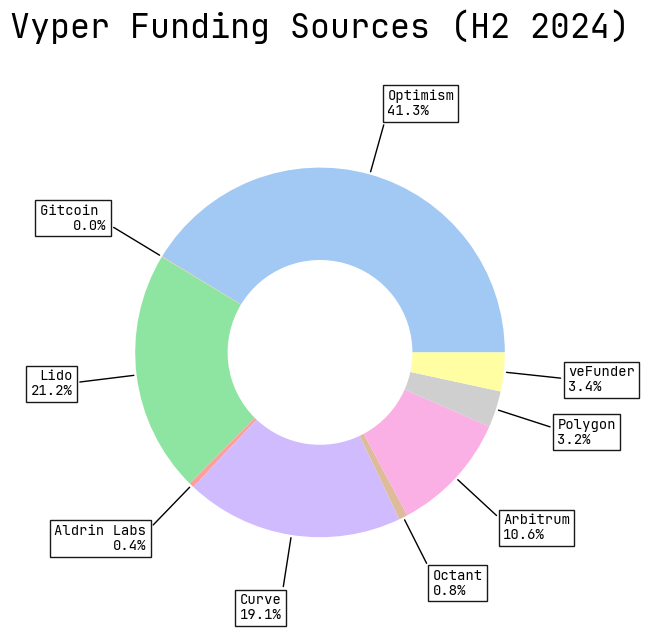
\includegraphics[width=\columnwidth]{charts/revenue.png}
			\end{column}
			\begin{column}{0.55\textwidth}
				\setbeamercolor{itemize item}{fg=vyperviolet}
				\setbeamercolor{itemize subitem}{fg=vyperviolet}
				\setbeamercolor{itemize subsubitem}{fg=vyperviolet}
				\begin{itemize}
					\item Sustainable grant funding is \textbf{diversified funding}. We seek to increase our sources of funding to avoid relying on any single funder.
					\vspace{0.5em}
					\item We are working to establish relationships and trust with funders to ensure more consistent and sizeable funding in the future
					\vspace{0.5em}
					\item Protocols using the language have been major funders. Increasing Vyper adoption helps ensure sustainable funding
				\end{itemize}
			\end{column}
		\end{columns}
	\end{frame}
	
	% Grant Funding Slide
	\begin{frame}
		\frametitle{Targeted Grants}
		\begin{tikzpicture}[remember picture,overlay]
			\foreach \x/\y/\title/\items [count=\i] in {
				0/0/{Public Goods Funding}/{Optimism RPGF, Octant, Gitcoin, EF, ENS, VeFunder,  Giveth, Dev Tooling Guild},
				1/0/{L2 Ecosystem Grants}/{Arbitrum, Optimism, Polygon, Scroll, Sonic Labs, Manta, Taiko},
				0/1/{Protocols (Rev Share/Grants) }/{Curve, Lido, Yearn, Frax, Aldrin Labs, Drips},
				1/1/{Non-web3 Grants}/{Academic Grants for R\&D, Python Foundation},
				0.5/2/{Direct Donations}/{Benevity, Llamas NFT, Developers, KOLs}
			} {
				\node[anchor=north west, 
				fill=bubblecolor!70, 
				opacity=0.5,
				rounded corners, 
				text width=0.4\paperwidth,
				inner sep=10pt,
				minimum height=5em] 
				at ($(current page.north west)+(0.03\paperwidth+0.49\paperwidth*\x,-0.22\paperheight-0.25\paperheight*\y)$) 
				(bubble\i) {};
				
				\node[circle, 
				fill=vyperviolet, 
				text=numbertextcolor, 
				font=\bfseries, 
				minimum size=1.5em] 
				at ($(bubble\i.north west)+(0.5em,-0.5em)$) 
				{\i};
				
				\node[anchor=north west, 
				font=\bfseries, 
				text width=0.4\paperwidth] 
				at ($(bubble\i.north west)+(2em,-0.5em)$) 
				{\title};
				
				\node[anchor=north west, 
				font=\footnotesize, 
				text width=0.4\paperwidth] 
				at ($(bubble\i.north west)+(0.5em,-2.5em)$) 
				{\items};
			}
		\end{tikzpicture}
	\end{frame}
	
	\begin{frame}
		\frametitle{Funding Sources (Commercial)}
		\begin{tikzpicture}[remember picture,overlay]
			\foreach \x/\y/\title/\items [count=\i] in {
				0/0/{Consulting}/{Code reviews, personalized assistance, advice on best practices, introductions to builders \& auditors},
				1/0/{Tooling Licensing}/{Introduce a freemium model for current (Titanoboa) or future (shadow events, debugger) tooling developed by the team},
				0/1/{Paid Partnerships}/{Protocols or L2s give funding in exchange for accelerated support of their chain and visibility (in docs, site \& socials)},
				1/1/{Token Allocations}/{Negotiate allocations from new protocols building with Vyper in exchange for assistance and/or promotion}
			} {
				\node[anchor=north west, 
				fill=bubblecolor!70, 
				opacity=0.5,
				rounded corners, 
				text width=0.4\paperwidth,
				inner sep=10pt,
				minimum height=7em] 
				at ($(current page.north west)+(0.03\paperwidth+0.49\paperwidth*\x,-0.22\paperheight-0.35\paperheight*\y)$) 
				(bubble\i) {};
				
				\node[circle, 
				fill=vyperviolet, 
				text=numbertextcolor, 
				font=\bfseries, 
				minimum size=1.5em] 
				at ($(bubble\i.north west)+(0.5em,-0.5em)$) 
				{\i};
				
				\node[anchor=north west, 
				font=\bfseries, 
				text width=0.4\paperwidth] 
				at ($(bubble\i.north west)+(2em,-0.5em)$) 
				{\title};
				
				\node[anchor=north west, 
				font=\footnotesize, 
				text width=0.4\paperwidth] 
				at ($(bubble\i.north west)+(0.5em,-2.5em)$) 
				{\items};
			}
		\end{tikzpicture}
	\end{frame}
\end{document}